\documentclass[11pt,a4paper]{article}

\usepackage[T1]{fontenc}
\usepackage[utf8]{inputenc}
\usepackage{lmodern}
\usepackage{microtype}
\usepackage[a4paper,top=23mm,bottom=24mm,left=22mm,right=22mm,headheight=15pt]{geometry}
\usepackage{amsmath,amssymb}
\usepackage{xcolor}
\usepackage{booktabs,tabularx,longtable,array}
\usepackage{graphicx}
\usepackage{tikz}
\usetikzlibrary{arrows.meta,positioning,calc,fit,backgrounds,shapes.geometric,decorations.pathreplacing,angles,quotes}
\usepackage{hyperref}

\definecolor{Ink}{HTML}{25262A}
\definecolor{Muted}{HTML}{68707A}
\definecolor{Paper}{HTML}{F7F4EC}
\definecolor{Blue}{HTML}{315CD6}
\definecolor{BlueSoft}{HTML}{E8EEFF}
\definecolor{Teal}{HTML}{259B9A}
\definecolor{TealSoft}{HTML}{E5F5F3}
\definecolor{Orange}{HTML}{E89B31}
\definecolor{OrangeSoft}{HTML}{FFF1DC}
\definecolor{Purple}{HTML}{7653B5}
\definecolor{PurpleSoft}{HTML}{F0EAF9}
\definecolor{Red}{HTML}{C94C4C}
\definecolor{Green}{HTML}{34865A}
\definecolor{RuleGray}{HTML}{D8DADD}

\hypersetup{
  colorlinks=true,
  linkcolor=Blue,
  urlcolor=Teal,
  citecolor=Purple,
  pdftitle={Planform V2 - Algorithms, Rules, and 3D Reconstruction Mechanism},
  pdfauthor={Planform project},
  pdfsubject={Floorplan image analysis and digital-twin generation}
}

\makeatletter
\def\ps@planform{
  \def\@oddhead{\small\color{Muted}PLANFORM V2 - TECHNICAL REPORT\hfil}
  \def\@evenhead{\small\color{Muted}PLANFORM V2 - TECHNICAL REPORT\hfil}
  \def\@oddfoot{\small\color{Muted}Implementation snapshot: 187f3b8\hfil\thepage}
  \def\@evenfoot{\small\color{Muted}\thepage\hfil Implementation snapshot: 187f3b8}
}
\let\ps@plain\ps@planform
\makeatother
\pagestyle{planform}

\setlength{\leftmargini}{5.5mm}
\setlength{\leftmarginii}{5mm}
\renewcommand{\arraystretch}{1.18}
\setlength{\parindent}{0pt}
\setlength{\parskip}{5pt}

\newcommand{\Planform}{\textsc{Planform}}
\newcommand{\code}[1]{\texttt{#1}}
\newcommand{\R}{\mathbb{R}}
\newcommand{\ind}{\mathbf{1}}
\newcommand{\clamp}{\operatorname{clamp}}
\newcommand{\norm}[1]{\left\lVert #1\right\rVert}

\newenvironment{keybox}[1]{
  \par\medskip\noindent\begin{minipage}{\textwidth}
  \color{Blue}\hrule height 0.8pt\vspace{1.6mm}\textbf{#1}\par\smallskip\color{Ink}
}{
  \vspace{1.3mm}\color{Blue}\hrule height 0.8pt\end{minipage}\par\medskip
}
\newenvironment{warningbox}[1]{
  \par\medskip\noindent\begin{minipage}{\textwidth}
  \color{Orange}\hrule height 0.8pt\vspace{1.6mm}\textbf{#1}\par\smallskip\color{Ink}
}{
  \vspace{1.3mm}\color{Orange}\hrule height 0.8pt\end{minipage}\par\medskip
}
\newenvironment{algorithmblock}[1]{
  \par\medskip\noindent\begin{minipage}{\textwidth}
  \color{Ink!55}\hrule height 0.6pt\vspace{1.4mm}\textbf{#1}\par\smallskip\color{Ink}
}{
  \vspace{1.2mm}\color{Ink!55}\hrule height 0.6pt\end{minipage}\par\medskip
}

\tikzset{
  flow/.style={rounded corners=2mm,draw=Ink!55,fill=white,thick,minimum height=9mm,text width=28mm,align=center,font=\small},
  flowblue/.style={flow,draw=Blue,fill=BlueSoft},
  flowteal/.style={flow,draw=Teal,fill=TealSoft},
  floworange/.style={flow,draw=Orange,fill=OrangeSoft},
  arrow/.style={-{Latex[length=2.5mm]},thick,draw=Ink!60},
  wall/.style={draw=Ink,line width=4.2pt,line cap=rect},
  thinwall/.style={draw=Ink,line width=2.6pt,line cap=rect},
  detect/.style={draw=Blue,line width=1.4pt},
  sample/.style={circle,fill=Purple,inner sep=1.2pt},
  note/.style={font=\scriptsize,align=center,text=Muted}
}

\begin{document}

\hypersetup{pageanchor=false}
\begin{titlepage}

\begin{tikzpicture}[remember picture,overlay]
  \fill[Paper] (current page.south west) rectangle (current page.north east);
  \fill[Blue] (current page.north west) rectangle ([yshift=-12mm]current page.north east);
  \fill[Teal] ([xshift=-34mm]current page.south east) rectangle (current page.north east);
  \draw[Blue!20,line width=18mm] ([xshift=-12mm,yshift=48mm]current page.south west) -- ([xshift=78mm,yshift=48mm]current page.south west);
  \draw[Orange!75,line width=5mm] ([xshift=24mm,yshift=29mm]current page.south west) -- ([xshift=110mm,yshift=29mm]current page.south west);
\end{tikzpicture}

\vspace*{26mm}
{\color{Blue}\Large\bfseries PLANFORM V2}\par
\vspace{5mm}
{\fontsize{28}{34}\selectfont\bfseries\color{Ink}
Algorithms, Rules, and\\[1mm]
3D Reconstruction Mechanism}\par
\vspace{7mm}
{\Large\color{Muted}A detailed implementation report with formulas, schemes, and geometric constructions}\par

\vspace{17mm}
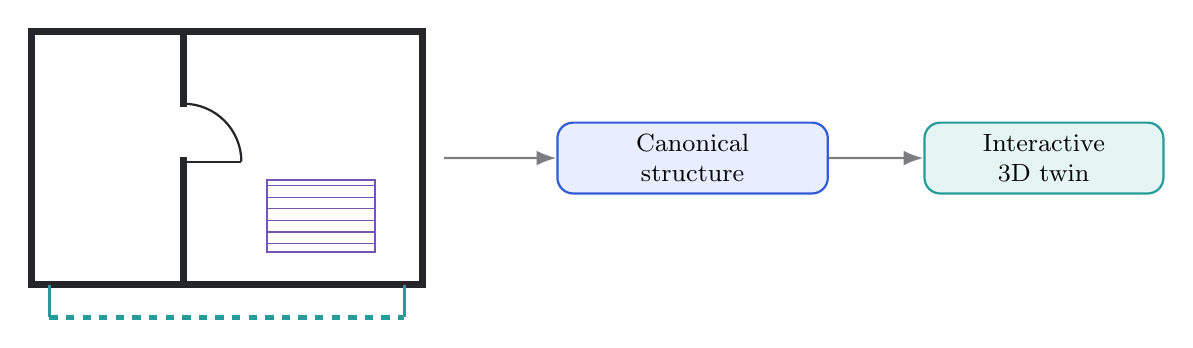
\begin{tikzpicture}[scale=0.92]
  \draw[thinwall] (0,0) -- (5.4,0) -- (5.4,3.5) -- (0,3.5) -- cycle;
  \draw[thinwall] (2.1,0) -- (2.1,1.7);
  \draw[thinwall] (2.1,2.5) -- (2.1,3.5);
  \draw[thinwall] (2.1,1.7) -- (2.1,1.72);
  \draw[Ink,line width=0.8pt] (2.1,1.7) -- (2.9,1.7);
  \draw[Ink,line width=0.8pt] (2.1,2.5) arc[start angle=90,end angle=0,radius=0.8];
  \draw[Purple,line width=0.8pt] (3.25,0.45) rectangle (4.75,1.45);
  \foreach \y in {0.57,0.73,0.89,1.05,1.21,1.37} \draw[Purple,line width=0.45pt] (3.25,\y) -- (4.75,\y);
  \draw[Teal,line width=1.6pt,dashed] (0.25,-0.45) -- (5.15,-0.45);
  \draw[Teal,line width=1.0pt] (0.25,-0.45) -- (0.25,0);
  \draw[Teal,line width=1.0pt] (5.15,-0.45) -- (5.15,0);
  \coordinate (coverplan) at (5.4,1.75);
  \node[flowblue,right=17mm of coverplan,text width=32mm] (model) {Canonical\\structure};
  \draw[arrow] (5.7,1.75) -- (model.west);
  \node[flowteal,right=12mm of model,text width=28mm] (twin) {Interactive\\3D twin};
  \draw[arrow] (model.east) -- (twin.west);
\end{tikzpicture}

\vfill
\begin{tabularx}{\textwidth}{@{}lX@{}}
\textbf{Implementation} & \code{v2-geometry-bootstrap} / browser geometry fallback \\
\textbf{Code snapshot} & Commit \code{187f3b8} \\
\textbf{Report revision} & 1.0 \\
\textbf{Date} & 15 August 2026 \\
\end{tabularx}
\vspace{8mm}
\end{titlepage}

\pagenumbering{roman}
\hypersetup{pageanchor=true}
\section*{Executive summary}
\addcontentsline{toc}{section}{Executive summary}

\Planform{} converts a raster floorplan into an editable structural graph and derives an interactive 3D model from that graph. The current implementation is a deterministic computer-vision pipeline executed in the browser. It is not a trained semantic model and does not contain a coordinate-specific rule for the validation residence.

The analyser combines five kinds of evidence:

\begin{enumerate}
  \item dark-stroke geometry and estimated stroke thickness;
  \item local wall continuity and wall-to-wall topology;
  \item explicit opening symbols, especially the door leaf and swing arc;
  \item cross-floor consistency for shared stair shafts;
  \item lower-confidence contextual fallback when direct symbols are degraded.
\end{enumerate}

The image axes are not assumed to be the building axes. Each plan region receives an estimated dominant rotation, is deskewed into a local orthogonal frame, and is then analysed. The plan-review overlay is transformed back to the source image, while the canonical geometry and floor texture stay deskewed for the 3D scene.

\begin{keybox}{Most important implementation boundary}
The current system supports a rectilinear floorplan that is globally rotated on the page. It does not yet fully vectorize buildings containing many diagonal walls, curved walls, or perspective distortion. In other words, it is image-axis invariant but not yet a general arbitrary-angle architectural vectorizer.
\end{keybox}

\tableofcontents
\listoffigures
\clearpage
\pagenumbering{arabic}

\section{System architecture}

The application separates source interpretation, canonical structure, and rendering. This avoids storing a mesh as the primary result. A wall remains a wall with endpoints, thickness, confidence, and openings; the viewer can then derive any suitable mesh representation.

\begin{figure}[htbp]
\centering
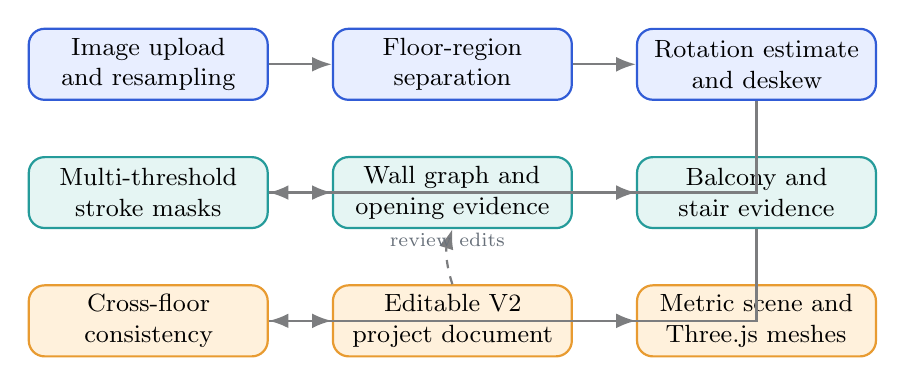
\begin{tikzpicture}[node distance=7mm and 8mm]
  \node[flowblue] (upload) {Image upload\\and resampling};
  \node[flowblue,right=of upload] (regions) {Floor-region\\separation};
  \node[flowblue,right=of regions] (rotate) {Rotation estimate\\and deskew};
  \node[flowteal,below=of upload] (masks) {Multi-threshold\\stroke masks};
  \node[flowteal,right=of masks] (walls) {Wall graph and\\opening evidence};
  \node[flowteal,right=of walls] (features) {Balcony and\\stair evidence};
  \node[floworange,below=of masks] (cross) {Cross-floor\\consistency};
  \node[floworange,right=of cross] (doc) {Editable V2\\project document};
  \node[floworange,right=of doc] (scene) {Metric scene and\\Three.js meshes};
  \draw[arrow] (upload) -- (regions);
  \draw[arrow] (regions) -- (rotate);
  \draw[arrow] (rotate) |- (masks);
  \draw[arrow] (masks) -- (walls);
  \draw[arrow] (walls) -- (features);
  \draw[arrow] (features) |- (cross);
  \draw[arrow] (cross) -- (doc);
  \draw[arrow] (doc) -- (scene);
  \draw[arrow,dashed] (doc.north) to[bend left=18] node[above,note]{review edits} (walls.south);
\end{tikzpicture}
\caption{Implemented analysis and reconstruction pipeline.}
\label{fig:pipeline}
\end{figure}

The principal modules are listed in Table~\ref{tab:modules}.

\begin{table}[htbp]
\centering
\caption{Code ownership by processing stage.}
\label{tab:modules}
\small
\begin{tabularx}{\textwidth}{@{}>{\bfseries\raggedright\arraybackslash}p{52mm}X@{}}
\toprule
Module & Responsibility \\
\midrule
\code{app/page.tsx} & Upload validation, pixel extraction, orchestration, review interface, and texture creation. \\
\code{app/plan-regions.ts} & Separation of disconnected floorplans and user-adjustable source regions. \\
\code{app/structure-detector.ts} & Rotation, masks, walls, openings, balconies, stairs, room estimate, confidence, and pixel-to-scene conversion. \\
\code{app/floorplan-document.ts} & Canonical schema, issues, edits, undo, level ordering, and project validation. \\
\code{app/scene-geometry.ts} & Stairwell cuts, slab fragments, stair connections, and scene footprint. \\
\code{app/twin-viewer.tsx} & Wall, window, stair, balcony, slab, and texture meshes. \\
\code{app/project-storage.ts} & IndexedDB storage and JSON import/export. \\
\bottomrule
\end{tabularx}
\end{table}

\section{Input model and raster preprocessing}

\subsection{Accepted source and analysis resolution}

The UI accepts JPEG, PNG, and WebP files up to 20 MB. Let the decoded image size be $W_0\times H_0$. The analysis scale is
\begin{equation}
s=\min\left(1,\frac{1280}{\max(W_0,H_0)}\right),\qquad
W=\max(1,\operatorname{round}(sW_0)),\quad
H=\max(1,\operatorname{round}(sH_0)).
\end{equation}
Smaller images are not enlarged. The 1280-pixel cap preserves one-pixel stair treads and door arcs better than the earlier 900-pixel cap while keeping mobile memory bounded.

\subsection{Luminance and Otsu threshold}

For an RGB pixel $p=(R,G,B)$, the detector uses
\begin{equation}
Y(p)=0.299R+0.587G+0.114B.
\end{equation}
Transparent pixels with $\alpha\leq 32$ are ignored. Otsu's method selects the gray value $t^*$ that maximizes the between-class variance
\begin{equation}
t^*=\arg\max_t\;\omega_0(t)\omega_1(t)\left[\mu_0(t)-\mu_1(t)\right]^2.
\end{equation}
The strong threshold is then brightened slightly and clamped:
\begin{equation}
T_s=\clamp(t^*+18,105,188).
\end{equation}
Two more permissive masks are retained:
\begin{equation}
T_m=\min(210,T_s+40),\qquad T_f=\min(205,T_s+26).
\end{equation}
$T_s$ identifies wall cores, $T_m$ preserves thinner door and stair evidence, and $T_f$ supports fine window strokes.

\subsection{Paper-bound correction}

Rows are sampled for pixels with $Y>205$. A row remains part of the paper when at least 8\% of its samples are paper-like. This removes large dark phone or browser bars without rejecting a legitimate row that is mostly occupied by a thick facade wall.

\section{Separating multiple floorplans}

The region detector operates on a coarse occupancy grid with $C=56$ columns and
\begin{equation}
R=\max\left(28,\operatorname{round}\left(56\frac{H}{W}\right)\right)
\end{equation}
rows. For grid cell $g$, sampled every two source pixels,
\begin{equation}
O(g)=\ind\left[\frac{\#\{p\in g:Y(p)<220\}}{\#\{p\in g\}}>0.035\right].
\end{equation}
The occupancy mask receives a $3\times3$ dilation and is split into four-connected components.

\begin{figure}[htbp]
\centering
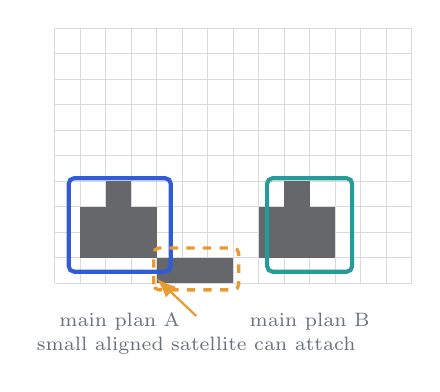
\begin{tikzpicture}[scale=0.72]
  \draw[step=0.45cm,RuleGray,very thin] (0,0) grid (6.3,4.5);
  \foreach \x/\y in {1/1,2/1,3/1,1/2,2/2,3/2,2/3,8/1,9/1,10/1,8/2,9/2,10/2,9/3,4/0,5/0,6/0} {
    \fill[Ink!70] (\x*0.45,\y*0.45) rectangle ++(0.45,0.45);
  }
  \draw[Blue,line width=1.5pt,rounded corners=2pt] (0.25,0.2) rectangle (2.05,1.85);
  \draw[Teal,line width=1.5pt,rounded corners=2pt] (3.75,0.2) rectangle (5.25,1.85);
  \draw[Orange,line width=1.2pt,dashed,rounded corners=2pt] (1.75,-0.12) rectangle (3.25,0.62);
  \node[note,below] at (1.15,-0.35) {main plan A};
  \node[note,below] at (4.5,-0.35) {main plan B};
  \node[note,below] at (2.5,-0.78) {small aligned satellite can attach};
  \draw[arrow,Orange] (2.5,-0.58) -- (1.8,0.08);
\end{tikzpicture}
\caption{Coarse connected components separate similarly sized floorplans while allowing a nearby smaller balcony or label component to attach to its host.}
\label{fig:regions}
\end{figure}

For component $a$ and candidate host $b$, define non-overlap gaps $g_x,g_y$ and
\begin{equation}
d(a,b)=\sqrt{g_x^2+g_y^2}.
\end{equation}
The component can attach only when it is aligned in at least one direction, is no more than 48\% of the host's occupied cells, and satisfies
\begin{equation}
d(a,b)\leq \max\left(2,\min\left(4,\operatorname{round}(0.18\min(w_b,h_b))\right)\right).
\end{equation}
Main components require at least 22 occupied cells and a grid box of at least $6\times6$. Up to four regions are returned, sorted visually from top to bottom and then left to right.

\begin{algorithmblock}{Algorithm 1 - Floor-region proposal}
\begin{enumerate}
  \item Convert the source image to the coarse occupancy grid $O$.
  \item Dilate $O$ by one grid cell and extract four-connected components.
  \item Remove tiny components; sort remaining components by occupied-cell count.
  \item Attach only aligned, nearby, substantially smaller satellite components.
  \item If brochure material creates extra groups, prefer plan-sized central groups.
  \item Return at most four padded normalized source rectangles.
\end{enumerate}
\end{algorithmblock}

Page position is never used directly as floor elevation. For exactly two regions, when exactly one has a detected outdoor platform, that plan is suggested as the upper level. The suggestion remains an unresolved review issue until the user confirms or reorders it.

\section{Dominant orientation and deskewing}

\subsection{Rotation score}

Let $\mathcal P$ contain dark pixels with at least three supported cells in their $3\times3$ neighborhood. Let $m$ be the smaller region dimension and
\begin{equation}
\mathcal D=\left\{\max(7,0.035m),\;\max(12,0.075m),\;\max(18,0.13m)\right\}.
\end{equation}
For candidate angle $\theta$, define orthogonal unit vectors
\begin{equation}
u_\theta=(\cos\theta,\sin\theta),\qquad
v_\theta=(-\sin\theta,\cos\theta).
\end{equation}
Let $h(q)=1$ when the dark mask has support within one pixel of $q$. With increasing weights $w_d\in\{1,2,3\}$ for longer distances, the implemented score is equivalent to
\begin{equation}
S(\theta)=\sum_{p\in\mathcal P}\sum_{d\in\mathcal D}w_d
\left[h(p+du_\theta)+h(p-du_\theta)+h(p+dv_\theta)+h(p-dv_\theta)\right].
\label{eq:rotation}
\end{equation}
The search covers integer angles $\theta\in[-44^\circ,45^\circ]$.

\begin{figure}[htbp]
\centering
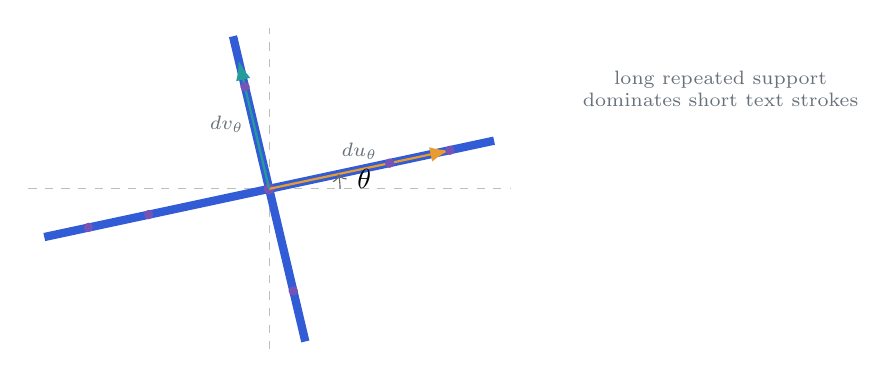
\begin{tikzpicture}[scale=1.02]
  \coordinate (p) at (0,0);
  \coordinate (xaxis) at (2,0);
  \coordinate (udir) at (2.25,0.48);
  \draw[Ink!30,dashed] (-3,0)--(3,0);
  \draw[Ink!30,dashed] (0,-2)--(0,2);
  \draw[Blue,line width=3pt] (-2.8,-0.6)--(2.8,0.6);
  \draw[Blue,line width=3pt] (-0.45,1.9)--(0.45,-1.9);
  \fill[Purple] (p) circle (2pt);
  \draw[arrow,Orange] (p)--(udir) node[midway,above,note]{$d u_\theta$};
  \draw[arrow,Teal] (p)--(-0.38,1.6) node[midway,left,note]{$d v_\theta$};
  \draw pic[draw=Ink!70,->,"$\theta$",angle eccentricity=1.35,angle radius=9mm] {angle=xaxis--p--udir};
  \foreach \x/\y in {-2.25/-0.48,-1.5/-0.32,1.5/0.32,2.25/0.48,-0.3/1.27,0.3/-1.27} \node[sample] at (\x,\y) {};
  \node[note,right=8mm] at (3,1.25) {long repeated support\\dominates short text strokes};
\end{tikzpicture}
\caption{Rotation is estimated from repeated support in two perpendicular directions, not from the source image axes.}
\label{fig:rotation}
\end{figure}

The best angle is rejected and replaced by $0^\circ$ when
\begin{equation}
|\theta^*|\leq1^\circ\quad\text{or}\quad S(\theta^*)\leq1.045S(0).
\end{equation}
This snap rule avoids resampling an already aligned drawing because of asymmetric rasterization.

\subsection{Stroke-preserving inverse mapping}

The deskewed destination point $q$ samples source coordinates
\begin{equation}
p=c+R_{\theta^*}(q-c),\qquad
R_\theta=\begin{bmatrix}\cos\theta&-\sin\theta\\\sin\theta&\cos\theta\end{bmatrix},
\end{equation}
where $c$ is the source-region center. Instead of bilinear interpolation, the darkest of the four neighboring source pixels is selected. This is a deliberate morphology-preserving choice for one-pixel arcs and rails.

\begin{algorithmblock}{Algorithm 2 - Rotation-normalized analysis}
\begin{enumerate}
  \item Build a strong dark mask in the proposed source region.
  \item Evaluate Equation~\eqref{eq:rotation} from $-44^\circ$ through $45^\circ$.
  \item Apply the snap-to-zero rule.
  \item If nonzero, inverse-map source pixels into a deskewed analysis canvas using darkest-neighbor sampling.
  \item Run the structural detector in the local orthogonal frame.
  \item Rotate overlays back onto the original image; keep canonical 3D geometry deskewed.
\end{enumerate}
\end{algorithmblock}

\begin{warningbox}{Scope of invariance}
This process removes one global rotation. It does not infer a separate angle for every wall. Therefore a rotated rectangular plan is supported, but a plan with many intrinsic diagonal or curved walls remains only partially represented.
\end{warningbox}

\section{Wall extraction and topology}

\subsection{Run masks and connected stroke components}

In each local principal direction, a dark run must have length
\begin{equation}
L_{\min}=\max(12,\operatorname{round}(0.06m))
\end{equation}
and at least 72\% dark support across its run after allowing a one-pixel interruption. Connected components are retained only when
\begin{equation}
\frac{\text{length}}{\max(1,\text{thickness})}\geq2.2.
\end{equation}
Components are split wherever full-thickness support disappears. This is essential when a one-pixel dimension line touches a thick wall.

The nominal wall thickness is the length-weighted 66th percentile
\begin{equation}
\tau_w=Q^{(L)}_{0.66}\left(\{\tau_i\}\right),
\end{equation}
computed from sufficiently long segments and clamped to $[2,0.07m]$ pixels.

\begin{figure}[htbp]
\centering
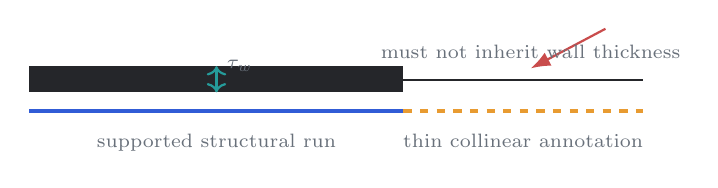
\begin{tikzpicture}[scale=0.95]
  \fill[Ink] (0,0) rectangle (5.0,0.35);
  \draw[Ink,line width=0.7pt] (5.0,0.17)--(8.2,0.17);
  \draw[Blue,line width=1.3pt] (0,-0.25)--(5.0,-0.25);
  \draw[Orange,line width=1.3pt,dashed] (5.0,-0.25)--(8.2,-0.25);
  \draw[<->,Teal,thick] (2.5,0)--(2.5,0.35) node[right,note]{$\tau_w$};
  \node[note,below] at (2.5,-0.42) {supported structural run};
  \node[note,below] at (6.6,-0.42) {thin collinear annotation};
  \draw[arrow,Red] (7.7,0.85)--(6.7,0.32) node[above,note]{must not inherit wall thickness};
\end{tikzpicture}
\caption{Cross-section support separates a real wall from an attached dimension line.}
\label{fig:falsewall}
\end{figure}

\subsection{Structural acceptance rules}

A raw candidate must satisfy thickness $\tau_i\geq\max(2,0.32\tau_w)$, length at least $0.06m$, and density at least 0.32. It then survives when at least one of the following holds:

\begin{itemize}
  \item $L_i\geq0.32m$;
  \item it connects to a perpendicular candidate within a tolerance proportional to $\tau_w$;
  \item it is a thick short junction fragment;
  \item it has a collinear continuation across a plausible door-sized gap.
\end{itemize}

For collinear continuation, line separation must be small. The gap must not exceed $\max(16,0.14m)$; one member must have length at least $0.24m$; and the current fragment must have length at least $0.09m$. This recovers partitions interrupted by door symbols.

\subsection{Anchor recovery and false-tail trimming}

Collinear structural segments are grouped and rescanned through their estimated cross-section. Solid support above 48\% creates wall anchors. Exterior groups may be rescanned across the whole footprint edge; interior groups are limited to observed extents.

After walls are built, a second cross-section analysis may trim exactly one unsupported interior tail. Trimming is forbidden for exterior walls, walls already containing openings, and very thin walls. The retained end must terminate at a perpendicular joint. These constraints remove the false living-room/kitchen divider caused by a dimension line without deleting a legitimate faint partition.

\begin{algorithmblock}{Algorithm 3 - Structural wall graph}
\begin{enumerate}
  \item Mark long runs in both local principal directions.
  \item Extract elongated connected components and split them by cross-section support.
  \item Merge collinear overlap and estimate $\tau_w$ by weighted quantile.
  \item Apply thickness, density, length, junction, and doorway-continuation rules.
  \item Recover solid anchors through a local rescan.
  \item Cluster collinear segments into walls and retain bounded gaps as opening candidates.
  \item Trim a single unsupported annotation tail only under strict topology constraints.
\end{enumerate}
\end{algorithmblock}

\section{Opening detection: doors and windows}

\subsection{Candidate wall gaps}

Let a gap run from local wall coordinate $a$ to $b$, with width $g=b-a$. It is ignored when
\begin{equation}
g\leq\max(3,0.75\tau_w).
\end{equation}
Large gaps are also bounded relative to the wall or footprint span so that two unrelated collinear walls are not automatically joined.

\subsection{Door symbol model}

The door classifier tests both gap endpoints as hinge $h$, both sides of the wall, and leaf angles
\begin{equation}
\phi\in\{55^\circ,60^\circ,\ldots,105^\circ\}.
\end{equation}
Let $e$ be the closed direction along the gap and $n$ the wall normal. A candidate leaf direction is
\begin{equation}
q_\phi=e\cos\phi+\sigma n\sin\phi,\qquad\sigma\in\{-1,+1\}.
\end{equation}
The leaf support is
\begin{equation}
s_L=\frac{1}{N_L}\sum_{i=1}^{N_L}H\left(h+r_iq_\phi\right),
\end{equation}
where $H$ tests dark support within a tolerance $\max(1,0.24\tau_w)$ and $r_i$ samples the leaf from 2/12 to 12/12 of the gap width.

For radius scale $\rho\in\{0.84,0.92,1.00\}$, arc support is
\begin{equation}
s_A=\max_\rho\frac{1}{N_A}\sum_{j=1}^{N_A}
H\left(h+\rho g\left[e\cos\alpha_j+\sigma n\sin\alpha_j\right]\right),
\qquad \alpha_j\in\left[\frac{2\phi}{14},\phi\right].
\end{equation}
The combined symbol score is
\begin{equation}
s_D=0.72\sqrt{s_Ls_A}+0.28\min(s_L,s_A).
\label{eq:door}
\end{equation}

\begin{figure}[htbp]
\centering
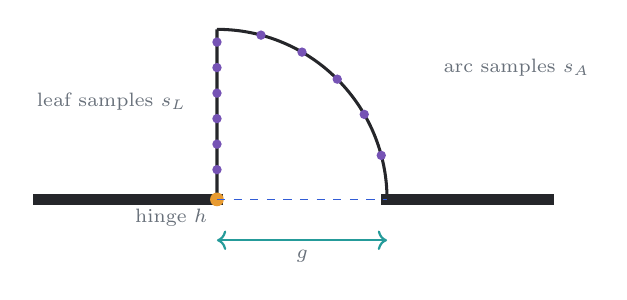
\begin{tikzpicture}[scale=1.08]
  \draw[wall] (-3,0)--(-0.9,0);
  \draw[wall] (1.1,0)--(3,0);
  \coordinate (h) at (-0.9,0);
  \draw[Ink,line width=1.2pt] (h)--(-0.9,2.0);
  \draw[Ink,line width=1.1pt] (1.1,0) arc[start angle=0,end angle=90,radius=2.0];
  \draw[<->,Teal,thick] (-0.9,-0.48)--(1.1,-0.48) node[midway,below,note]{$g$};
  \fill[Orange] (h) circle (2.3pt) node[below left,note]{hinge $h$};
  \foreach \y in {0.35,0.65,0.95,1.25,1.55,1.85} \node[sample] at (-0.9,\y) {};
  \foreach \a in {15,30,45,60,75} \node[sample] at ({-0.9+2*cos(\a)},{2*sin(\a)}) {};
  \node[note,right] at (1.65,1.55) {arc samples $s_A$};
  \node[note,left] at (-1.15,1.15) {leaf samples $s_L$};
  \draw[Blue,dashed] (h)--(1.1,0);
\end{tikzpicture}
\caption{Rotation-normalized door model. A high-confidence door requires both the radial leaf and the swing arc.}
\label{fig:door}
\end{figure}

A gap receives direct \code{symbol} evidence only when
\begin{equation}
s_D\geq0.46,\qquad s_L\geq0.42,\qquad s_A\geq0.34.
\end{equation}
Its confidence is
\begin{equation}
C_D=\clamp(0.62+0.34s_D,0.68,0.97).
\end{equation}
The geometric mean in Equation~\eqref{eq:door} prevents either a straight furniture edge or an isolated curve from producing a strong door by itself.

\subsection{Window and fallback evidence}

The window score searches a band of width $2.4\tau_w$ around the wall for fine strokes parallel to the gap. Strong parallel support on an exterior wall is classified as a window. Interior windows are treated as uncommon.

If the complete leaf-and-arc symbol is unavailable, a gap may still be classified from perpendicular run length, general curved-pixel density, and parallel strokes. Evidence is recorded as shown in Table~\ref{tab:evidence}.

\begin{table}[htbp]
\centering
\caption{Opening evidence hierarchy.}
\label{tab:evidence}
\begin{tabularx}{\textwidth}{@{}>{\ttfamily}p{23mm}p{38mm}X@{}}
\toprule
Value & Interpretation & Use \\
\midrule
symbol & Leaf plus swing arc & Highest-confidence door recognition. \\
geometry & Stroke arrangement & Windows and partial but structurally supported doors. \\
context & Bounded interior gap & Lower-confidence door fallback when the symbol is degraded. \\
\bottomrule
\end{tabularx}
\end{table}

\begin{keybox}{Removed exception}
The detector does not promote the opening closest to the center of a balcony. The validation residence now passes only when its balcony door is classified from leaf-and-arc \code{symbol} evidence.
\end{keybox}

\begin{algorithmblock}{Algorithm 4 - Opening classification}
\begin{enumerate}
  \item Locate a bounded gap between collinear structural wall sections.
  \item Evaluate every hinge endpoint, wall side, leaf angle, and arc-radius scale.
  \item If the joint leaf-and-arc thresholds pass, return a \code{symbol} door.
  \item Otherwise test strong parallel fine strokes for an exterior window.
  \item Otherwise test partial perpendicular and curved geometry.
  \item Permit a bounded internal \code{context} door only at reduced confidence.
\end{enumerate}
\end{algorithmblock}

\section{Balcony and terrace detection}

Outdoor platforms are recognized from geometry rather than language. For each local footprint side, the analyser searches for an external rail and two roughly perpendicular supports.

For a horizontal facade of width $W_f$ and height $H_f$, an external horizontal rail at depth $d$ must satisfy
\begin{equation}
0.10H_f\leq d\leq0.62H_f,
\qquad
\frac{\text{overlap}(\text{rail},\text{facade})}{W_f}\geq0.44.
\end{equation}
Each side support must span at least $0.55d$, two supports are required, and their separation must be at least $0.40W_f$. The vertical-side test is the transposed equivalent. At most two highest-confidence outdoor areas are retained.

\begin{figure}[htbp]
\centering
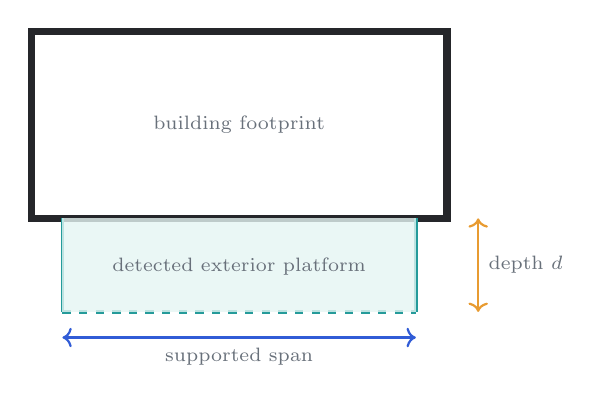
\begin{tikzpicture}[scale=0.88]
  \draw[thinwall] (-3,0)--(3,0)--(3,2.7)--(-3,2.7)--cycle;
  \draw[Teal,line width=1.3pt,dashed] (-2.55,-1.35)--(2.55,-1.35);
  \draw[Teal,line width=1.3pt] (-2.55,-1.35)--(-2.55,0);
  \draw[Teal,line width=1.3pt] (2.55,-1.35)--(2.55,0);
  \fill[TealSoft,opacity=.8] (-2.55,-1.35) rectangle (2.55,0);
  \draw[<->,Orange,thick] (3.45,0)--(3.45,-1.35) node[midway,right,note]{depth $d$};
  \draw[<->,Blue,thick] (-2.55,-1.72)--(2.55,-1.72) node[midway,below,note]{supported span};
  \node[note] at (0,-0.7) {detected exterior platform};
  \node[note] at (0,1.35) {building footprint};
\end{tikzpicture}
\caption{Balcony evidence consists of an exterior rail with two side supports and sufficient facade overlap.}
\label{fig:balcony}
\end{figure}

In 3D, the platform's pixel span and depth are converted to scene units and constrained to touch the corresponding slab edge. The renderer adds the platform, guard panels, rails, and posts.

\section{Stair detection and floor-to-floor alignment}

\subsection{Plan-symbol detection}

Thin candidate rails are consolidated when their lengths lie between $0.052m$ and $0.52m$ and their thickness is no more than $\max(4,0.82\tau_w)$. A rail pair must have the same local axis and satisfy
\begin{align}
0.065m &\leq \Delta_{\text{rail}}\leq0.31m,\\
\text{overlap}_{\text{run}}&\geq0.045m,\\
0.52\Delta_{\text{rail}}&\leq L_{\text{run}}\leq4.8\Delta_{\text{rail}}.
\end{align}
At least two thin cross-stroke centers must occur between the rails. If their median spacing is $\widetilde{\Delta}$, the step estimate is
\begin{equation}
N_s=\clamp\left(\operatorname{round}\left(\frac{L_{\text{run}}}{\max(3,\widetilde{\Delta})}\right),\max(5,N_c),16\right),
\end{equation}
where $N_c$ is the number of observed cross-stroke centers. Candidates with fewer than six final steps or implausibly large boxes are rejected.

\begin{figure}[htbp]
\centering
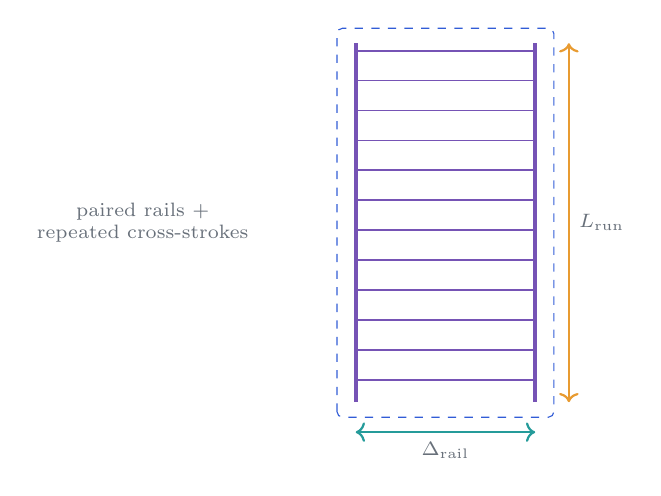
\begin{tikzpicture}[scale=0.95]
  \draw[Purple,line width=1.5pt] (-1.2,-2.4)--(-1.2,2.4);
  \draw[Purple,line width=1.5pt] (1.2,-2.4)--(1.2,2.4);
  \foreach \y in {-2.1,-1.7,-1.3,-0.9,-0.5,-0.1,0.3,0.7,1.1,1.5,1.9,2.3} {
    \draw[Purple,line width=0.65pt] (-1.2,\y)--(1.2,\y);
  }
  \draw[<->,Teal,thick] (-1.2,-2.8)--(1.2,-2.8) node[midway,below,note]{$\Delta_{\text{rail}}$};
  \draw[<->,Orange,thick] (1.65,-2.4)--(1.65,2.4) node[midway,right,note]{$L_{\text{run}}$};
  \draw[Blue,dashed,rounded corners=2pt] (-1.45,-2.6) rectangle (1.45,2.6);
  \node[note,left=10mm] at (-1.45,0) {paired rails +\\repeated cross-strokes};
\end{tikzpicture}
\caption{The stair detector validates paired rails using repeated tread strokes and size constraints.}
\label{fig:stairdetect}
\end{figure}

Connected strokes beside an off-center detected flight may expand the shaft to include a return flight or winders. A solid wall column is rejected by limiting the acceptable dark proportion along the expansion scan.

\subsection{Shared shaft normalization}

For stair $s$ in footprint $F=(x_F,y_F,w_F,h_F)$, define normalized center
\begin{equation}
\bar c(s,F)=\left(\frac{x_s+w_s/2-x_F}{w_F},\frac{y_s+h_s/2-y_F}{h_F}\right).
\end{equation}
The highest-confidence upper-floor shaft is compared with lower-floor candidates of the same run axis. The closest candidate is aligned only when
\begin{equation}
\norm{\bar c_{\text{lower}}-\bar c_{\text{upper}}}_2\leq0.22.
\end{equation}
The upper normalized box is projected into the lower footprint. The upper plan is authoritative because its slab opening is usually drawn more completely.

\subsection{Half-paced 3D construction}

Let lower and upper slab elevations be $z_0$ and $z_1$. The landing elevation is
\begin{equation}
z_L=\frac{z_0+z_1}{2}.
\end{equation}
The lower and upper flights occupy opposite lanes inside the upper-floor shaft opening. Each flight receives approximately one step per 0.19 m of rise, clamped to 6--11 steps. The final upper tread is placed exactly at the upper opening edge rather than ending at shorter source linework.

\begin{figure}[htbp]
\centering
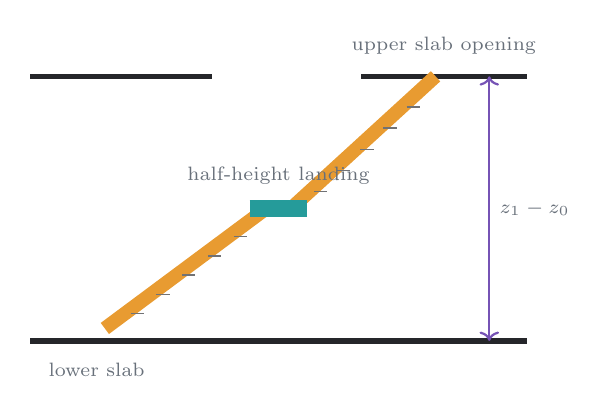
\begin{tikzpicture}[x=1.05cm,y=1.05cm]
  \draw[Ink,line width=2pt] (-3,0)--(3,0);
  \draw[Ink,line width=2pt] (-3,3.2)--(-0.8,3.2);
  \draw[Ink,line width=2pt] (1.0,3.2)--(3,3.2);
  \draw[Orange,line width=5pt] (-2.1,0.15)--(-0.15,1.6);
  \draw[Orange,line width=5pt] (0.15,1.6)--(1.9,3.2);
  \draw[Teal,line width=6pt] (-0.35,1.6)--(0.35,1.6);
  \foreach \t in {0.16,0.32,0.48,0.64,0.80} {
    \draw[Ink!65,line width=0.5pt] ({-2.1+1.95*\t},{0.15+1.45*\t-0.05})--({-2.1+1.95*\t+0.16},{0.15+1.45*\t-0.05});
    \draw[Ink!65,line width=0.5pt] ({0.15+1.75*\t},{1.6+1.6*\t-0.05})--({0.15+1.75*\t+0.16},{1.6+1.6*\t-0.05});
  }
  \draw[<->,Purple,thick] (2.55,0)--(2.55,3.2) node[midway,right,note]{$z_1-z_0$};
  \node[note,below] at (-2.2,-0.15) {lower slab};
  \node[note,above] at (2.0,3.35) {upper slab opening};
  \node[note,above] at (0,1.78) {half-height landing};
\end{tikzpicture}
\caption{Elevation scheme for the generated half-paced stair connection. In plan, the two flights occupy opposite lanes of one shared shaft.}
\label{fig:halfpace}
\end{figure}

\section{Room topology and confidence}

\subsection{Room-count estimate}

Walls are rasterized onto a $72\times72$ binary grid and the outside border is closed. Four-connected flood fill counts empty components with area at least
\begin{equation}
0.012\times72^2\approx62\text{ cells}.
\end{equation}
The result is clamped to 1--20. This is a topology-derived room estimate, not recognition of room purpose or labels.

\subsection{Structure confidence}

Let $N_w$ be walls, $N_t$ topology-supported walls, and $N_o$ openings. Let $I_b$ and $I_s$ indicate at least one outdoor area and stair. The implemented confidence is
\begin{align}
C_{\text{raw}}={}&0.46+\min(0.24,0.018N_w)+\min(0.10,0.012N_t)\\
&+\min(0.08,0.012N_o)+0.03I_b+0.025I_s,\\
C={}&\clamp(C_{\text{raw}},C_{\min},0.94),
\end{align}
where $C_{\min}=0.58$ for at least four walls and $0.38$ otherwise.

\begin{warningbox}{Interpretation of confidence}
These scores rank evidence inside the deterministic pipeline. They are not probabilities calibrated on a large labeled population. A wall confidence below 0.70 creates a review warning.
\end{warningbox}

\section{Pixel geometry to the 3D digital twin}

\subsection{Provisional scale}

Until one known measurement is supplied, the scene width is fixed to 10 m. For footprint width $W_f$ and height $H_f$,
\begin{equation}
k=\frac{10}{W_f}\quad\text{m/pixel},\qquad
D=\clamp(kH_f,4.2,15)\quad\text{m}.
\end{equation}
For footprint center $(c_x,c_y)$, image point $(x,y)$ maps to
\begin{equation}
X=k(x-c_x),\qquad Z=k(y-c_y).
\end{equation}

\refstepcounter{table}
\begin{center}
Table~\thetable: Current default dimensions before scale calibration.
\end{center}
\begin{tabularx}{\textwidth}{@{}Xr@{}}
\toprule
Quantity & Value \\
\midrule
Level width & 10.00 m \\
Floor-to-floor elevation & 3.05 m \\
Base / upper ceiling height & 2.70 m / 2.55 m \\
Door height & 2.12 m \\
Window height / sill & 1.30 m / 0.90 m \\
Converted wall thickness & clamped to 0.10--0.42 m \\
\bottomrule
\end{tabularx}

Every level receives a \code{scale-needed} issue because these defaults provide coherent navigation, not survey-grade dimensions.

\subsection{Wall meshes and openings}

For scene wall endpoints $A=(X_1,Z_1)$ and $B=(X_2,Z_2)$,
\begin{equation}
L=\norm{B-A}_2,\qquad
\psi=\operatorname{atan2}(Z_2-Z_1,X_2-X_1).
\end{equation}
The renderer creates oriented boxes rotated by $-\psi$. Openings split the wall into body intervals. A door receives only a header above 2.12 m. A window receives a sill, header, and translucent glass panel.

\begin{figure}[htbp]
\centering
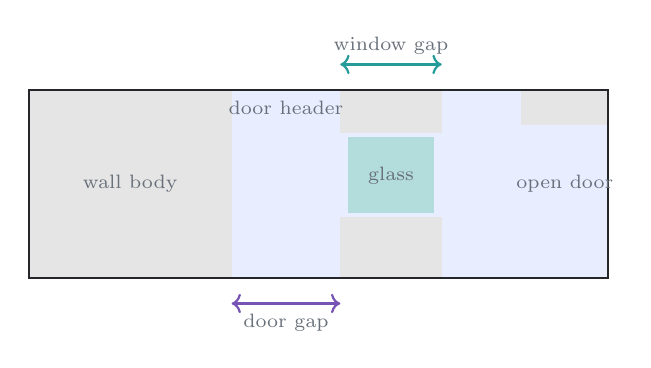
\begin{tikzpicture}[scale=0.92]
  \fill[BlueSoft] (-4,0) rectangle (4,2.6);
  \fill[Ink!12] (-4,0) rectangle (-1.2,2.6);
  \fill[Ink!12] (0.3,0) rectangle (1.7,0.85);
  \fill[Ink!12] (0.3,2.0) rectangle (1.7,2.6);
  \fill[Teal!35] (0.4,0.9) rectangle (1.6,1.95);
  \fill[Ink!12] (2.8,2.12) rectangle (4,2.6);
  \draw[Ink,line width=0.8pt] (-4,0) rectangle (4,2.6);
  \draw[<->,Purple,thick] (-1.2,-0.35)--(0.3,-0.35) node[midway,below,note]{door gap};
  \draw[<->,Teal,thick] (0.3,2.95)--(1.7,2.95) node[midway,above,note]{window gap};
  \node[note] at (-2.6,1.3) {wall body};
  \node[note] at (-0.45,2.35) {door header};
  \node[note] at (1.0,1.42) {glass};
  \node[note] at (3.4,1.3) {open door};
\end{tikzpicture}
\caption{Wall geometry is generated as boxes around door and window intervals rather than drawing openings only as textures.}
\label{fig:wallmesh}
\end{figure}

\subsection{Slab opening, texture, and viewer controls}

The upper slab is split into left, right, back, and front pieces around the stairwell rectangle. Each piece receives UV coordinates into the same deskewed floorplan crop. Balcony extents contribute to camera framing. Wall opacity and exploded separation affect rendering only; they do not mutate the canonical project.

\section{Canonical document, review, and persistence}

The V2 project document stores source metadata, ordered levels, detected structures, issues, edits, and a preview. Each level carries provenance \code{geometry} and \code{topology}; the runtime is explicitly \code{geometry-fallback}.

Current review operations are:
\begin{itemize}
  \item remove a detected wall;
  \item add a centered door or window to a selected wall;
  \item undo wall removal or opening addition;
  \item rename, reorder, or reverse levels;
  \item expand or shrink a source region;
  \item realign adjacent stair shafts;
  \item select visible levels and change wall opacity.
\end{itemize}

Projects are written to IndexedDB after a 220 ms debounce. The newest local project can be resumed on the same browser and device. JSON export/import provides a portable \code{.planform.json} backup. A saved project is not silently re-analysed after detector updates; the source must be uploaded again to use a newer algorithm.

\section{Failure modes and deterministic safeguards}

\small
\begin{longtable}{@{}p{34mm}p{54mm}p{64mm}@{}}
\caption{Known failure modes and current safeguards.}\label{tab:failures}\\
\toprule
Failure mode & Likely effect & Current safeguard \\
\midrule
\endfirsthead
\toprule
Failure mode & Likely effect & Current safeguard \\
\midrule
\endhead
Heavy JPEG blur & Thin arcs and rails disappear & Multi-threshold masks and darkest-neighbor deskew sampling. \\
Dimension line touches wall & False wall extension & Full-thickness support splitting and one-tail topology trim. \\
Door interrupts short partition & Wall fragment discarded & Collinear doorway-continuation rule and anchor recovery. \\
Global page rotation & Axis-run detector misses walls & Dominant-angle estimate and local deskewed frame. \\
Oblique photograph & Nonuniform wall angles & Not yet corrected; use a screenshot or flat scan. \\
Many diagonal/curved walls & Missing or simplified structure & Documented limitation; requires arbitrary-angle tracing. \\
Furniture resembles a door & False opening & Door requires both leaf and arc for \code{symbol} evidence. \\
Window resembles exterior gap & Door/window confusion & Parallel fine-stroke score and exterior-wall context. \\
Different stair linework per floor & Shifted shafts & Normalized upper-shaft projection when distance $\leq0.22$. \\
No physical dimension & Incorrect absolute size & Explicit \code{scale-needed} issue and provisional scale. \\
Analysis exception & Empty workspace & Single low-confidence fallback region. \\
\bottomrule
\end{longtable}

\section{Validation strategy}

The repository validates behavior at four levels:

\begin{enumerate}
  \item \textbf{Synthetic geometry:} thick walls, door arcs, windows, false dimension tails, stairs, slab cuts, and half-paced connections.
  \item \textbf{Private floorplan corpus:} seven user-supplied fixtures when present locally, with integrity hashes and expected level counts.
  \item \textbf{Validation residence:} balcony, both stairs, balcony swing door, entrance-bedroom partition, floor order, and absence of the false living-room/kitchen wall.
  \item \textbf{Rotation regression:} the validation residence rotated by $9^\circ$ and a synthetic swing-door plan rotated by $11^\circ$.
\end{enumerate}

The balcony-door assertion requires \code{evidence = symbol}; therefore the test cannot pass because of balcony position alone. The private fixtures are excluded from the public repository and deployment and are explicitly not approved for model training or public redistribution.

\section{Current limitations and next architecture}

\begin{enumerate}
  \item The pipeline is classical geometry/topology, not a trained semantic wall/door/furniture model.
  \item One global rotation is corrected, but multiple intrinsic wall-angle families and curved walls are not fully traced.
  \item Perspective rectification is absent.
  \item OCR is absent; labels and written dimensions do not establish semantics or scale.
  \item Furniture, cupboards, toilets, sinks, and tables remain floor-texture detail rather than individual 3D entities.
  \item The UI accepts raster images, not PDF.
  \item Room count is approximate and room function is unknown.
  \item IndexedDB persistence is local, not cross-device cloud sync.
  \item The 3D stair is a generated half-paced archetype, not a complete reconstruction of every stair type.
\end{enumerate}

The recommended future architecture is an ensemble:
\begin{equation}
\begin{aligned}
\mathcal E={}&\text{semantic segmentation}
\;\oplus\;\text{arbitrary-angle vector tracing}\\
&\oplus\;\text{OCR/scale extraction}
\;\oplus\;\text{current topology validator}.
\end{aligned}
\end{equation}
The existing geometry layer should remain independent. It can reject a visually plausible semantic prediction when the result fails wall continuity, opening placement, or cross-floor consistency.

\section{Rule hierarchy and conclusion}

The implemented decision hierarchy is shown in Figure~\ref{fig:hierarchy}.

\begin{figure}[htbp]
\centering
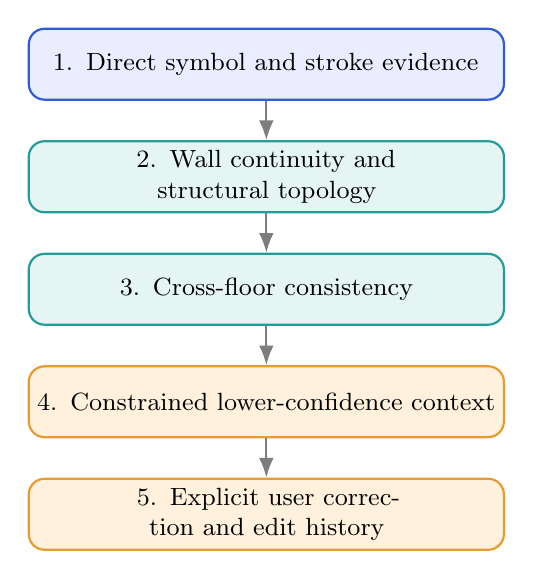
\begin{tikzpicture}[node distance=5mm]
  \node[flowblue,text width=58mm] (direct) {1. Direct symbol and stroke evidence};
  \node[flowteal,text width=58mm,below=of direct] (topology) {2. Wall continuity and structural topology};
  \node[flowteal,text width=58mm,below=of topology] (cross) {3. Cross-floor consistency};
  \node[floworange,text width=58mm,below=of cross] (context) {4. Constrained lower-confidence context};
  \node[floworange,text width=58mm,below=of context] (user) {5. Explicit user correction and edit history};
  \draw[arrow] (direct)--(topology);
  \draw[arrow] (topology)--(cross);
  \draw[arrow] (cross)--(context);
  \draw[arrow] (context)--(user);
\end{tikzpicture}
\caption{Evidence hierarchy: direct image evidence dominates context, and the user remains authoritative.}
\label{fig:hierarchy}
\end{figure}

\Planform{} now has a reproducible structural foundation: relative thresholds adapt to image size, door classification can be traced to an explicit symbol score, page rotation is normalized before tracing, and cross-floor rules enforce physical consistency. The system remains intentionally honest about the difference between a geometry-based proposal and a trained semantic digital-twin extractor.

\clearpage
\appendix
\section{Compact parameter reference}

\begin{longtable}{@{}p{53mm}p{31mm}p{70mm}@{}}
\caption{Principal implemented parameters.}\label{tab:params}\\
\toprule
Parameter & Value & Purpose \\
\midrule
\endfirsthead
\toprule
Parameter & Value & Purpose \\
\midrule
\endhead
Maximum analysis side & 1280 px & Mobile memory / thin-stroke preservation. \\
Region grid & 56 columns & Multi-floor component detection. \\
Occupied-cell ratio & 0.035 & Coarse dark-content threshold. \\
Max floor regions & 4 & Current intake bound. \\
Rotation search & $[-44^\circ,45^\circ]$ & Global plan deskew. \\
Rotation snap & $1^\circ$ or 4.5\% & Avoid needless resampling. \\
Minimum long run & $\max(12,0.06m)$ & Wall candidate evidence. \\
Run dark density & 0.72 & Tolerate one-pixel interruptions. \\
Component aspect ratio & 2.2 & Reject compact text/furniture blobs. \\
Wall-thickness quantile & 0.66 weighted & Estimate nominal stroke thickness. \\
Structural density & 0.32 & Reject sparse candidate components. \\
Door angle search & $55^\circ$--$105^\circ$ & Support varied door-leaf drawings. \\
Door radius scales & 0.84, 0.92, 1.00 & Support imperfect arcs. \\
Door score threshold & 0.46 & Require joint leaf and arc evidence. \\
Balcony depth & 0.10--0.62 footprint & Locate exterior rail. \\
Balcony overlap & 0.44 & Require facade alignment. \\
Stair rail separation & 0.065--0.31 $m$ & Bound shaft width. \\
Stair step count & 5--16 & Reject implausible line clusters. \\
Cross-floor stair distance & 0.22 normalized & Align shared shaft. \\
Room grid & $72\times72$ & Topology flood fill. \\
Low-confidence wall warning & 0.70 & Trigger human review. \\
Maximum structure confidence & 0.94 & Avoid false certainty. \\
\bottomrule
\end{longtable}

\clearpage
\section{Canonical entity summary}

\refstepcounter{table}
\begin{center}
Table~\thetable: Principal entities stored in the V2 project.
\end{center}
\begin{tabularx}{\textwidth}{@{}p{27mm}p{47mm}X@{}}
\toprule
Entity & Core fields & Meaning \\
\midrule
Source region & normalized rectangle, name, confidence & One visual floorplan on the uploaded image. \\
Wall & endpoints, thickness, openings, confidence & Structural boundary in deskewed pixel coordinates. \\
Opening & kind, offset, width, confidence, evidence & Door or window interval along one wall. \\
Outdoor area & side, rectangle, confidence & Balcony or terrace attached to a footprint edge. \\
Stair & shaft box, run axis, step count, confidence & Plan-level stair proposal. \\
Level & order, elevation, source region, structure & One building storey. \\
Issue & code, severity, entity, resolved state & Required or recommended human review. \\
Edit & kind, before, after, timestamp & Reversible user correction history. \\
\bottomrule
\end{tabularx}

\vfill
\begin{center}
\color{Muted}\small
End of report. The formulas and thresholds in this document describe the implementation at code snapshot \code{187f3b8}.
\end{center}

\end{document}
